%% bare_conf.tex
%% V1.4b
%% 2015/08/26
%% by Michael Shell
%% See:
%% http://www.michaelshell.org/
%% for current contact information.
%%
%% This is a skeleton file demonstrating the use of IEEEtran.cls
%% (requires IEEEtran.cls version 1.8b or later) with an IEEE
%% conference paper.
%%
%% Support sites:
%% http://www.michaelshell.org/tex/ieeetran/
%% http://www.ctan.org/pkg/ieeetran
%% and
%% http://www.ieee.org/
%%*************************************************************************
%% Legal Notice:
%% This code is offered as-is without any warranty either expressed or
%% implied; without even the implied warranty of MERCHANTABILITY or
%% FITNESS FOR A PARTICULAR PURPOSE! 
%% User assumes all risk.
%% In no event shall the IEEE or any contributor to this code be liable for
%% any damages or losses, including, but not limited to, incidental,
%% consequential, or any other damages, resulting from the use or misuse
%% of any information contained here.
%%
%% All comments are the opinions of their respective authors and are not
%% necessarily endorsed by the IEEE.
%%
%% This work is distributed under the LaTeX Project Public License (LPPL)
%% ( http://www.latex-project.org/ ) version 1.3, and may be freely used,
%% distributed and modified. A copy of the LPPL, version 1.3, is included
%% in the base LaTeX documentation of all distributions of LaTeX released
%% 2003/12/01 or later.
%% Retain all contribution notices and credits.
%% ** Modified files should be clearly indicated as such, including  **
%% ** renaming them and changing author support contact information. **
%%*************************************************************************


% *** Authors should verify (and, if needed, correct) their LaTeX system  ***
% *** with the testflow diagnostic prior to trusting their LaTeX platform ***
% *** with production work. The IEEE's font choices and paper sizes can   ***
% *** trigger bugs that do not appear when using other class files.       ***                          
% The testflow support page is at:
% http://www.michaelshell.org/tex/testflow/

\documentclass[conference]{IEEEtran}
% Some Computer Society conferences also require the compsoc mode option,
% but others use the standard conference format.
%
% If IEEEtran.cls has not been installed into the LaTeX system files,
% manually specify the path to it like:
% \documentclass[conference]{../sty/IEEEtran}

\usepackage{booktabs}
\usepackage{balance}

\newcommand{\ra}[1]{\renewcommand{\arraystretch}{#1}}

\usepackage[usenames,dvipsnames]{color}
\newcommand{\todo}[1]
  {{\scriptsize \textbf{\color{red} {#1}}}}



% Some very useful LaTeX packages include:
% (uncomment the ones you want to load)


% *** MISC UTILITY PACKAGES ***
%
%\usepackage{ifpdf}
% Heiko Oberdiek's ifpdf.sty is very useful if you need conditional
% compilation based on whether the output is pdf or dvi.
% usage:
% \ifpdf
%   % pdf code
% \else
%   % dvi code
% \fi
% The latest version of ifpdf.sty can be obtained from:
% http://www.ctan.org/pkg/ifpdf
% Also, note that IEEEtran.cls V1.7 and later provides a builtin
% \ifCLASSINFOpdf conditional that works the same way.
% When switching from latex to pdflatex and vice-versa, the compiler may
% have to be run twice to clear warning/error messages.


\usepackage{listings}



% *** CITATION PACKAGES ***
%
\usepackage{cite}
% cite.sty was written by Donald Arseneau
% V1.6 and later of IEEEtran pre-defines the format of the cite.sty package
% \cite{} output to follow that of the IEEE. Loading the cite package will
% result in citation numbers being automatically sorted and properly
% "compressed/ranged". e.g., [1], [9], [2], [7], [5], [6] without using
% cite.sty will become [1], [2], [5]--[7], [9] using cite.sty. cite.sty's
% \cite will automatically add leading space, if needed. Use cite.sty's
% noadjust option (cite.sty V3.8 and later) if you want to turn this off
% such as if a citation ever needs to be enclosed in parenthesis.
% cite.sty is already installed on most LaTeX systems. Be sure and use
% version 5.0 (2009-03-20) and later if using hyperref.sty.
% The latest version can be obtained at:
% http://www.ctan.org/pkg/cite
% The documentation is contained in the cite.sty file itself.
\lstset{language=Java}
\definecolor{dkgreen}{rgb}{0,0.5,0}
\definecolor{dkred}{rgb}{0.5,0,0}
\definecolor{gray}{rgb}{0.5,0.5,0.5}
\lstset{
basicstyle=\ttfamily\bfseries\scriptsize,
  morekeywords={virtualinvoke}, 
  keywordstyle=\color{blue},
  ndkeywordstyle=\color{red},
  commentstyle=\color{dkred},
  stringstyle=\color{dkgreen},
  numbers=left,
  breaklines=true,
  numberstyle=\ttfamily\footnotesize\color{gray},
  stepnumber=1,
  numbersep=10pt,
  backgroundcolor=\color{white},
  tabsize=4,
  showspaces=false,
  frame=bt,
  showstringspaces=false,
  xleftmargin=.23in,
  moredelim=[is][\color{red}]{@}{@}, deletekeywords={}, captionpos=b, belowskip=1pt
}






% *** GRAPHICS RELATED PACKAGES ***
%
\ifCLASSINFOpdf
   \usepackage[pdftex]{graphicx}
  % declare the path(s) where your graphic files are
   \graphicspath{{images/}}
  % and their extensions so you won't have to specify these with
  % every instance of \includegraphics
   \DeclareGraphicsExtensions{.pdf,.jpeg,.png, .jpg}
\else
  % or other class option (dvipsone, dvipdf, if not using dvips). graphicx
  % will default to the driver specified in the system graphics.cfg if no
  % driver is specified.
  % \usepackage[dvips]{graphicx}
  % declare the path(s) where your graphic files are
  % \graphicspath{{../eps/}}
  % and their extensions so you won't have to specify these with
  % every instance of \includegraphics
  % \DeclareGraphicsExtensions{.eps}
\fi
% graphicx was written by David Carlisle and Sebastian Rahtz. It is
% required if you want graphics, photos, etc. graphicx.sty is already
% installed on most LaTeX systems. The latest version and documentation
% can be obtained at: 
% http://www.ctan.org/pkg/graphicx
% Another good source of documentation is "Using Imported Graphics in
% LaTeX2e" by Keith Reckdahl which can be found at:
% http://www.ctan.org/pkg/epslatex
%
% latex, and pdflatex in dvi mode, support graphics in encapsulated
% postscript (.eps) format. pdflatex in pdf mode supports graphics
% in .pdf, .jpeg, .png and .mps (metapost) formats. Users should ensure
% that all non-photo figures use a vector format (.eps, .pdf, .mps) and
% not a bitmapped formats (.jpeg, .png). The IEEE frowns on bitmapped formats
% which can result in "jaggedy"/blurry rendering of lines and letters as
% well as large increases in file sizes.
%
% You can find documentation about the pdfTeX application at:
% http://www.tug.org/applications/pdftex





% *** MATH PACKAGES ***
%
\usepackage{amsmath}
% A popular package from the American Mathematical Society that provides
% many useful and powerful commands for dealing with mathematics.
%
% Note that the amsmath package sets \interdisplaylinepenalty to 10000
% thus preventing page breaks from occurring within multiline equations. Use:
%\interdisplaylinepenalty=2500
% after loading amsmath to restore such page breaks as IEEEtran.cls normally
% does. amsmath.sty is already installed on most LaTeX systems. The latest
% version and documentation can be obtained at:
% http://www.ctan.org/pkg/amsmath





% *** SPECIALIZED LIST PACKAGES ***
%
%\usepackage{algorithmic}
% algorithmic.sty was written by Peter Williams and Rogerio Brito.
% This package provides an algorithmic environment fo describing algorithms.
% You can use the algorithmic environment in-text or within a figure
% environment to provide for a floating algorithm. Do NOT use the algorithm
% floating environment provided by algorithm.sty (by the same authors) or
% algorithm2e.sty (by Christophe Fiorio) as the IEEE does not use dedicated
% algorithm float types and packages that provide these will not provide
% correct IEEE style captions. The latest version and documentation of
% algorithmic.sty can be obtained at:
% http://www.ctan.org/pkg/algorithms
% Also of interest may be the (relatively newer and more customizable)
% algorithmicx.sty package by Szasz Janos:
% http://www.ctan.org/pkg/algorithmicx




% *** ALIGNMENT PACKAGES ***
%
%\usepackage{array}
% Frank Mittelbach's and David Carlisle's array.sty patches and improves
% the standard LaTeX2e array and tabular environments to provide better
% appearance and additional user controls. As the default LaTeX2e table
% generation code is lacking to the point of almost being broken with
% respect to the quality of the end results, all users are strongly
% advised to use an enhanced (at the very least that provided by array.sty)
% set of table tools. array.sty is already installed on most systems. The
% latest version and documentation can be obtained at:
% http://www.ctan.org/pkg/array


% IEEEtran contains the IEEEeqnarray family of commands that can be used to
% generate multiline equations as well as matrices, tables, etc., of high
% quality.




% *** SUBFIGURE PACKAGES ***
%\ifCLASSOPTIONcompsoc
%  \usepackage[caption=false,font=normalsize,labelfont=sf,textfont=sf]{subfig}
%\else
%  \usepackage[caption=false,font=footnotesize]{subfig}
%\fi
% subfig.sty, written by Steven Douglas Cochran, is the modern replacement
% for subfigure.sty, the latter of which is no longer maintained and is
% incompatible with some LaTeX packages including fixltx2e. However,
% subfig.sty requires and automatically loads Axel Sommerfeldt's caption.sty
% which will override IEEEtran.cls' handling of captions and this will result
% in non-IEEE style figure/table captions. To prevent this problem, be sure
% and invoke subfig.sty's "caption=false" package option (available since
% subfig.sty version 1.3, 2005/06/28) as this is will preserve IEEEtran.cls
% handling of captions.
% Note that the Computer Society format requires a larger sans serif font
% than the serif footnote size font used in traditional IEEE formatting
% and thus the need to invoke different subfig.sty package options depending
% on whether compsoc mode has been enabled.
%
% The latest version and documentation of subfig.sty can be obtained at:
% http://www.ctan.org/pkg/subfig




% *** FLOAT PACKAGES ***
%
%\usepackage{fixltx2e}
% fixltx2e, the successor to the earlier fix2col.sty, was written by
% Frank Mittelbach and David Carlisle. This package corrects a few problems
% in the LaTeX2e kernel, the most notable of which is that in current
% LaTeX2e releases, the ordering of single and double column floats is not
% guaranteed to be preserved. Thus, an unpatched LaTeX2e can allow a
% single column figure to be placed prior to an earlier double column
% figure.
% Be aware that LaTeX2e kernels dated 2015 and later have fixltx2e.sty's
% corrections already built into the system in which case a warning will
% be issued if an attempt is made to load fixltx2e.sty as it is no longer
% needed.
% The latest version and documentation can be found at:
% http://www.ctan.org/pkg/fixltx2e


%\usepackage{stfloats}
% stfloats.sty was written by Sigitas Tolusis. This package gives LaTeX2e
% the ability to do double column floats at the bottom of the page as well
% as the top. (e.g., "\begin{figure*}[!b]" is not normally possible in
% LaTeX2e). It also provides a command:
%\fnbelowfloat
% to enable the placement of footnotes below bottom floats (the standard
% LaTeX2e kernel puts them above bottom floats). This is an invasive package
% which rewrites many portions of the LaTeX2e float routines. It may not work
% with other packages that modify the LaTeX2e float routines. The latest
% version and documentation can be obtained at:
% http://www.ctan.org/pkg/stfloats
% Do not use the stfloats baselinefloat ability as the IEEE does not allow
% \baselineskip to stretch. Authors submitting work to the IEEE should note
% that the IEEE rarely uses double column equations and that authors should try
% to avoid such use. Do not be tempted to use the cuted.sty or midfloat.sty
% packages (also by Sigitas Tolusis) as the IEEE does not format its papers in
% such ways.
% Do not attempt to use stfloats with fixltx2e as they are incompatible.
% Instead, use Morten Hogholm'a dblfloatfix which combines the features
% of both fixltx2e and stfloats:
%
% \usepackage{dblfloatfix}
% The latest version can be found at:
% http://www.ctan.org/pkg/dblfloatfix


\usepackage{verbatim}
\usepackage{amsmath}
\usepackage{amsfonts}
\usepackage{amssymb}
\usepackage{graphicx}

% INCLUDE THIS
\usepackage{listings, lstautogobble}

% *** PDF, URL AND HYPERLINK PACKAGES ***
%
\usepackage{url}
% url.sty was written by Donald Arseneau. It provides better support for
% handling and breaking URLs. url.sty is already installed on most LaTeX
% systems. The latest version and documentation can be obtained at:
% http://www.ctan.org/pkg/url
% Basically, \url{my_url_here}.




% *** Do not adjust lengths that control margins, column widths, etc. ***
% *** Do not use packages that alter fonts (such as pslatex).         ***
% There should be no need to do such things with IEEEtran.cls V1.6 and later.
% (Unless specifically asked to do so by the journal or conference you plan
% to submit to, of course. )


% correct bad hyphenation here
\hyphenation{op-tical net-works semi-conduc-tor}

\usepackage{microtype}
\usepackage{lipsum}
\usepackage{multicol}
\usepackage{multirow}

\usepackage{array}
\usepackage{tabulary}
\newcolumntype{K}[1]{>{\arraybackslash}p{#1}}

\usepackage{array}
\newcolumntype{C}[1]{>{\centering\arraybackslash}m{#1}}
\newcolumntype{R}[1]{>{\raggedleft\arraybackslash}m{#1}}

\usepackage{adjustbox}

 
\pagenumbering{arabic}
\begin{document}
%
% paper title
% Titles are generally capitalized except for words such as a, an, and, as,
% at, but, by, for, in, nor, of, on, or, the, to and up, which are usually
% not capitalized unless they are the first or last word of the title.
% Linebreaks  can be used within to get better formatting as desired.
% Do not put math or special symbols in the title.
\title{Using a probabilistic model to predict bug fixes}


% author names and affiliations
% use a multiple column layout for up to three different
% affiliations


\author{\IEEEauthorblockN{Mauricio Soto}
\IEEEauthorblockA{School of Computer Science \\
Carnegie Mellon University\\
Pittsburgh, PA, USA\\
mauriciosoto@cmu.edu}
\and
\IEEEauthorblockN{Claire Le Goues}
\IEEEauthorblockA{School of Computer Science \\
Carnegie Mellon University\\
Pittsburgh, PA, USA\\
clegoues@cs.cmu.edu}




%\and
%\IEEEauthorblockN{James Kirk\\ and Montgomery Scott}
%\IEEEauthorblockA{Starfleet Academy\\
%San Francisco, California 96678--2391\\
%Telephone: (800) 555--1212\\
%Fax: (888) 555--1212}

}

% conference papers do not typically use \thanks and this command
% is locked out in conference mode. If really needed, such as for
% the acknowledgment of grants, issue a \IEEEoverridecommandlockouts
% after \documentclass

% for over three affiliations, or if they all won't fit within the width
% of the page, use this alternative format:
% 
%\author{\IEEEauthorblockN{Michael Shell\IEEEauthorrefmark{1},
%Homer Simpson\IEEEauthorrefmark{2},
%James Kirk\IEEEauthorrefmark{3}, 
%Montgomery Scott\IEEEauthorrefmark{3} and
%Eldon Tyrell\IEEEauthorrefmark{4}}
%\IEEEauthorblockA{\IEEEauthorrefmark{1}School of Electrical and Computer Engineering\\
%Georgia Institute of Technology,
%Atlanta, Georgia 30332--0250\\ Email: see http://www.michaelshell.org/contact.html}
%\IEEEauthorblockA{\IEEEauthorrefmark{2}Twentieth Century Fox, Springfield, USA\\
%Email: homer@thesimpsons.com}
%\IEEEauthorblockA{\IEEEauthorrefmark{3}Starfleet Academy, San Francisco, California 96678-2391\\
%Telephone: (800) 555--1212, Fax: (888) 555--1212}
%\IEEEauthorblockA{\IEEEauthorrefmark{4}Tyrell Inc., 123 Replicant Street, Los Angeles, California 90210--4321}}




% use for special paper notices
%\IEEEspecialpapernotice{(Invited Paper)}




% make the title area
\maketitle

% As a general rule, do not put math, special symbols or citations
% in the abstract
\begin{abstract}
Automatic Software Repair (APR) has significant potential to reduce software
maintenance costs by reducing the human effort required to localize and fix
bugs. State-of-the-art generate-and-validate 
APR techniques select between and instantiate various mutation operators
to construct candidate patches, informed largely by heuristic probability
distributions.  This may reduce effectiveness in terms of both efficiency and
output quality.  In practice, human developers
have many options in terms of how to edit code to fix bugs, some of which 
are far more common than others (e.g., deleting a line of code is more common
than adding a new class).
We  
mined the most recent 100 bug-fixing commits from each of the 500 most popular
Java projects in GitHub (the largest 
dataset to date) to
create a probabilistic model describing edit distributions.
We categorize, compare and evaluate the different mutation operators used in 
state-of-the-art approaches. 
We find that a probabilistic model-based APR approach 
patches bugs more quickly in the majority of bugs
studied, and that the resulting patches are of higher quality than those produced by
previous approaches. 
Finally, we mine association rules for
multi-edit source code changes, an understudied but important problem. 
We validate the
association rules by analyzing how much of our corpus can be built from them. Our evaluation
indicates that 84.6\% of the multi-edit patches from the corpus can be built from the association rules, while maintaining 90\% confidence. 
\end{abstract}


% no keywords




% For peer review papers, you can put extra information on the cover
% page as needed:
% \ifCLASSOPTIONpeerreview
% \begin{center} \bfseries EDICS Category: 3-BBND \end{center}
% \fi
%
% For peerreview papers, this IEEEtran command inserts a page break and
% creates the second title. It will be ignored for other modes.
\IEEEpeerreviewmaketitle



\section{Introduction} \label{introduction}

% no \IEEEPARstart
\looseness-1
Repairing bugs is one of the most 
resource-intensive tasks in 
software development~\cite{Weiss07,Tassey02,Britton13}.
%
Significant recent research effort has been dedicated to
building automatic program repair (APR) tools that are able to address
bugs in 
programs (e.g.~\cite{legoues12,kim2013,Weimer13,long15SPR,long16proph,debroy10,perkins09,wei10}).
%
One well-known class of repair techniques follows a 
\emph{generate-and-validate} approach (e.g., GenProg~\cite{legoues12}, 
Par~\cite{kim2013}, TrpAutoRepair~\cite{Qi13TrpAutoR},
Prophet~\cite{long16proph}, HDRepair~\cite{xuan16}, Angelix~\cite{Mechtaev2016},
Nopol~\cite{xuanNopol}), which takes as input a test suite, 
including at
least one failing test case exposing
a defect, and source code to be 
modified.  These approaches then \emph{generate} a large patch candidate space 
by applying 
mutation operators to the original source code and \emph{validate} each by
running the potentially patched program against the test suite, seeking a candidate that
leads the program to pass all tests. 

One key reason this is challenging is that the search space of possible edits
that can be applied to the original source code is infinite. To tackle this
problem, techniques limit themselves to a set of possible change types,
which we refer to broadly as ``Mutation operators''. 
There is a broad diversity of such operators used in automatic program repair, including deleting or inserting 
 statements~\cite{legoues12}, applying templates~\cite{kim2013}, transformation 
 schemas~\cite{long16proph,long15SPR}, or semantically-inferred code~\cite{nguyen13,Mechtaev2016,xuanNopol}.
 Given a potentially-faulty location (typically identified using off-the-shelf
fault localization, e.g., Tarantula~\cite{Jones02}), these
approaches then use heuristics or
heuristically-informed probability distributions to select between
mutation operators
to construct candidate patches.
%
Even with these efforts, the search space for possible edits remains vast; not
all bugs can be repaired; and many produced patches are of low quality.

Our intuition is that, in bug-fixing reality, human developers use certain mutation operators 
much more frequently than 
others (e.g., deleting a line is much more common than creating a new class), and we can use that knowledge to drive our search. In this paper, we therefore study and then simulate the behavior of human
developers to create patches. Our key supposition is that our approach can support a richer
search space constructed via more expressive mutation operators that are more
likely to produce high-quality patches.
%
Indeed, this idea has been
leveraged manually in the past to create more human-acceptable mutation
operators~\cite{kim2013} and to inform patch \emph{ranking} (rather than
construction)~\cite{xuan16,long16proph}.

% The APR search space, including the various mutation
% operators used by different techniques, has been growing in a relatively ad hoc 
% manner by the different approaches created in the latest years. We mitigate this effect by categorizing and comparing a superset of
% mutation operators in use in a number of 
% state-of-the-art approaches~\cite{legoues12,Weimer13,kim2013,long16proph}.

We mine bug fixing commits from 
the 500 most popular GitHub Java projects to model the selection probability of
the possible mutation operators based on 
empirical data that describes how human programmers fix their code.  We thus
categorize, compare, and validate a superset of
mutation operators in use in a number of 
state-of-the-art approaches~\cite{legoues12,Weimer13,kim2013,long16proph}. We then use this
model to inform a repair approach that chooses from the set of possible
operators based on these real-world
probabilities.
As a result, our work goes beyond prior work that leverages human bug
fixes in a program repair context~\cite{kim2013,xuan16,long16proph} by generalizing
to a broader and more expressive set of
mutation operators, and using a fully-automatically-mined model much 
earlier in the APR process, when
patch candidates are actually created.  
Furthermore, we propose and initially validate a new approach for modeling
multi-edit repairs based on mining previous rules from historical edit data, 
predicting from a given 
set of edits which operation should be applied
next.  This serves  as a first step towards
scalable traversal of the multi-edit patch space. 


We evaluate the predictive power of our mined model on its own, in terms of its
accuracy in predicting the operators used in real-world bug fixes. We demonstrate this algorithm both in terms of speed and quality with a full set of mutation
operators on a subset of real-world single-line defects~\cite{just14}, and we validate the quality of the patches found by our approach
in comparison to several previous state-of-the-art techniques. 

%
The primary contributions of this paper thus are:
\begin{itemize}
\item \textbf{Empirical model of single-edit repairs to Java code} mined
      from the 100 most recent bug fixes from the 500 most popular Java projects on
    GitHub. This study also provides a deeper
    understanding of which mutation operators are used to fix
    errors in source code, and the frequency of the mutation operators
    analyzed. 
	\item \textbf{New Repair Approach}, which uses mutation operators
    from multiple state-of-the-art approaches and
    the above-mentioned models to choose between them, favoring those more commonly
    used by human developers.  We validate the use of this model, as well as a
    good set of operators to use for expressive, high-quality repair.
    \item \textbf{Development and integration} of this approach for the Java
      programming language in a publicly-available tool that can apply the
      several different mutation operators, and the probabilistic model
      discussed in this study.
  \item \textbf{Comparative evaluation} of the new repair approach on real world bugs from well-known open source projects (independent of those used to inform model
    construction), as compared to several previous techniques. We independently evaluate patch quality using a held-out test
    suite. We conclude a technique based on a model informed by human behavior,
    finds patches more quickly than prior techniques that do not; that the
    patches are of comparatively higher quality; and that patch creation
    benefits from a diverse set of candidate mutation operators.
  \item \textbf{Multi-edit repair approach} A proposed technique, and an initial
    validation thereof, to construct 
    bug-fixing patches requiring several mutations by mining and then applying association
    rules from a large set of historical bug fixes. 
  \item \textbf{Code and data} that produced and were produced by our
    experiments, available at \url{FIXME}, to support reproducibility and
    extension. 
\end{itemize}

The rest of this paper proceeds as follows: We first outline
generate-and-validate repair and, in particular, 
categorize the mutation operators used in state-of-the-art
approaches (Section~\ref{background}). Section~\ref{buildingTheModel}
describes our approach to building probabilistic models of human 
edits for both single- and multi-edit bug fixes. Section~\ref{evaluation}
describes our evaluation. Section~\ref{relatedWork} describes
related work; Section~\ref{conclusion} concludes. 

\section{Generate-and-validate repair and operators} 
\label{background}

In this section, we outline generate and validate repair at a high level
(Section~\ref{sec-paradigm}), to provide the necessary background to understand this study.\footnote{We focus on relevant background in this section, and describe
  other techniques for automatic program repair in Section~\ref{relatedWork}.}
  We then detail and categorize the mutation operators used in prior approaches
  for syntactic program repair and that we model, mine, and leverage in our approach
(Section~\ref{categorization}).  
 
 
\subsection{Paradigm}
\label{sec-paradigm}


Figure~\ref{fig:generateandvalidate} outlines the general paradigm for generate-and-validate repair. This approach begins with two elements: buggy source code and a test suite. The test suite is comprised of passing
test cases to describe the correct program behavior, and failing test 
cases to expose the behavior to be repaired.

\begin{figure}[!h]
  \centering
    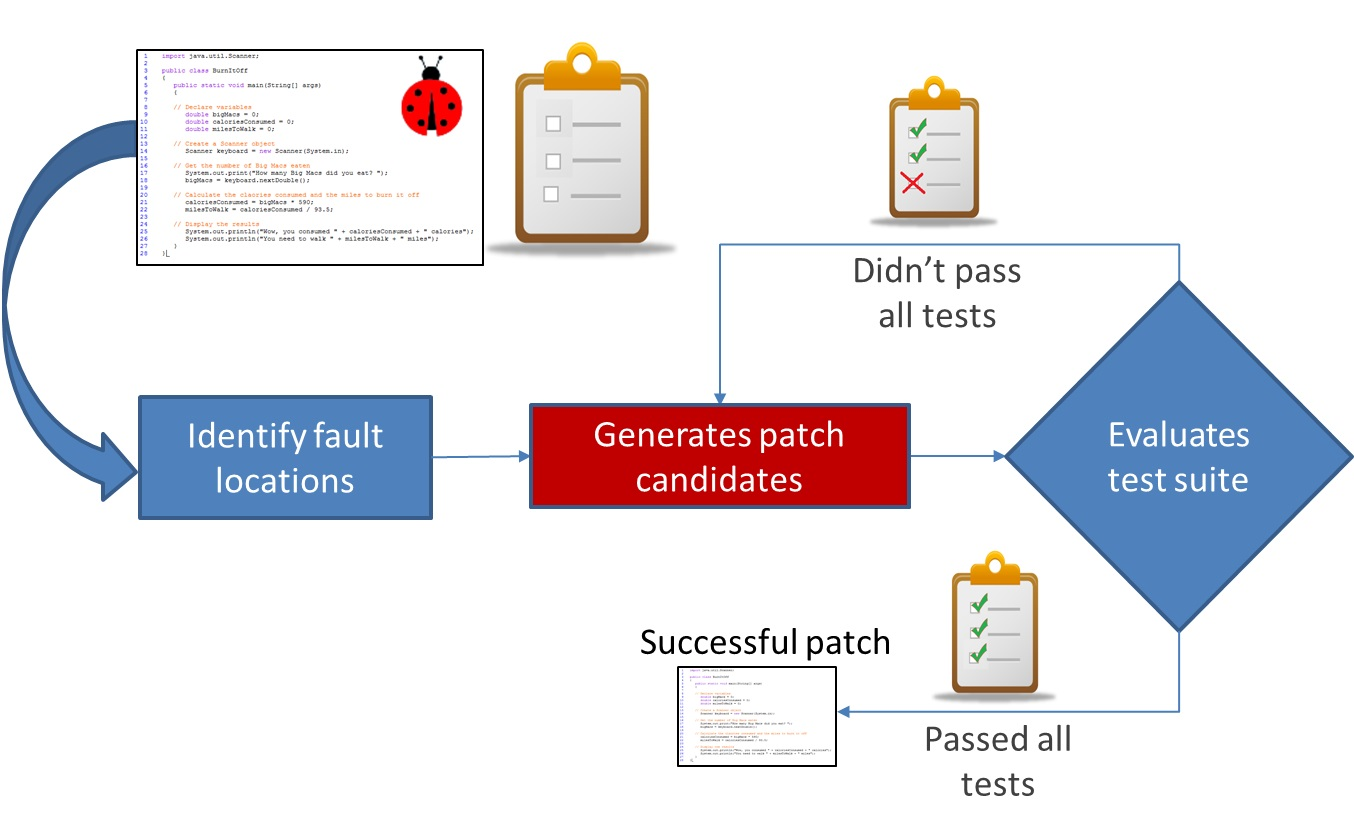
\includegraphics[width=\columnwidth]{Picture1}
  \caption{Generate-and-validate repair approach.}
  \label{fig:generateandvalidate}
\end{figure}

A generic generate-and-validate APR approach first
localizes the error to a smaller set of
candidate program statements (typically using an off-the-shelf statistical approach~\cite{Jones02}).  It
then constructs one or more candidate patches that seek to fix the buggy
behavior without breaking any previously-correct behavior.  
Techniques vary in (1) the mutation operators that they consider, (2) how they select
between those operators, and how they identify or
construct the fix code used to instantiate them, and (3) how they traverse
the search space otherwise.  
Most mutation operators (with the exception of deletion) require new code to
fill in ``holes.''  For example, an operator that replaces one statement with
another must select replacement code; an operator that wraps a statement
in a null check must select the object to be checked against null.
Syntactic approaches (e.g.,~\cite{legoues12Genprog,long16proph,kim2013,xuan16}) typically select this code from within the
same function, module, file, or program.  Semantic approaches instead use synthesis to
construct fix code.  
In both cases, heuristics inform code selection.  For example, some syntactic approaches
choose between fix code uniformly at random or using other set probability distributions~\cite{kim2013,legoues12Genprog}; others used learned
models to do so~\cite{long16proph}.  Semantic approaches use heuristics to
decide which program components should be made available to the synthesis
engine~\cite{Mechtaev2016,xuanNopol}. 

Once constructed of one or more such mutations, each candidate patch is
applied to the input program, which is then run on
one or more of the input test cases for evaluation.  If a patch leads the
program to 
pass all the test cases in the test suite, including those originally witnessing
the bug, it is presented as a likely repair for the bug. 
If not, the APR algorithm typically creates more candidate patches 
until it reaches a pre-defined resource limit. 
Here, too, search strategies vary: some techniques 
are explicitly single-edit~\cite{Qi13TrpAutoR,Weimer13,xuanNopol}; others use
random search strategies, like a random walk~\cite{debroy10} or genetic
programming~\cite{kim2013,legoues12,xuan16}.

\looseness-1
Patch quality is an important concern in APR research~\cite{Qi15}: Ideally,
created patches will generalize beyond the test cases used to inform their
construction~\cite{smith15}, and conform to other non-functional standards of
acceptability~\cite{fry2010,kim2013}.  Although assessing patch quality is an
unsolved research problem~\cite{monperrus14critical}, one mechanism for
objectively evaluating functional patch
correctness is to evaluate generated patches on a held-out test suite~\cite{smith15,legoues12Genprog}, separate
from the tests used to construct the patches. 
If the generated patch allows the program to pass all held-out tests, it is more likely to
\emph{generalize} to the desired but unwritten specification. If the patched
program fails any held-out tests, the patch is said to \emph{overfit} to 
the test suite that guided the repair. 


\subsection{Generate-and-validate mutation operators} 
\label{categorization}

We categorize mutation operators used from a cross
section of state-of-the-art approaches into two groups: 

\paragraph{Statement-Edit mutations}
One family of repair approaches, including GenProg~\cite{legoues12}, 
TrpAutoRepair~\cite{Qi13TrpAutoR}, and AE~\cite{Weimer13},
creates candidate 
patches by applying coarse-grained mutation operators (e.g. \emph{append}, \emph{delete}, or 
\emph{replace}) at the statement level. These prior techniques historically target the C programming language, where
a statement is a grammar nonterminal corresponding intuitively to blocks,
simple statements that terminate
with a semicolon, or compound statements corresponding to control flow or
loops. In Java, statements conceptually map to similar program elements, e.g. blocks,  while loops, or single-line
method calls. In these approaches, the statements being appended or replaced
typically come from within the project being modified. This is grounded in the
notion that source code has a high level of
redundancy~\cite{Hindle12Naturalness}. 

\paragraph{Template-based mutations}
Another family of approaches instantiates
predetermined templates, more complex than those in the first family, at applicable code locations.  This family includes PAR~\cite{kim2013}, 
SPR~\cite{long15SPR}, and 
Prophet~\cite{long16proph}.

PAR is the product of a study of a large number of 
human 
created patches, from which human annotators abstracted 10 different templates to cover
the most commonly-used changes in bug-fixing practice.
The 10 considered templates are detailed in the top section of Figure~\ref{approachTemplates}. In the interest of completeness, we also include six extra templates 
mentioned on the PAR website.\footnote{\url{https://sites.google.com/site/autofixhkust/home/fix-templates}} 
These extra templates provide new mutation operators drawn from human edits,
that help us compare to and
generalize the other approaches; they are shown in the middle segment of
Figure~\ref{approachTemplates}. 
SPR and Prophet use a set of transformation schemas,
shown in the bottom section of Figure~\ref{approachTemplates}.

\begin{figure}[ht]
  \centering
{\small
\begin{tabular}{ll}
\toprule
\multicolumn{2}{c}{PAR fix templates} \\
\midrule
Null Checker & Parameter Adder and Remover \\ 
Parameter Replacer & Expression Adder and Remover \\  
Method Replacer & Collection Size Checker \\
Expression Replacer &  Range Checker\\
Object Initializer & Class Cast Checker\\
\midrule
\multicolumn{2}{c}{PAR ``extra'' templates} \\
\midrule
Caster Mutator & Lower Bound Setter  \\
Castee Mutator & Upper Bound Setter  \\
Sequence Exchanger & Off-by-one Mutator\\
\midrule
\multicolumn{2}{c}{SPR transformation schema} \\
\midrule
Condition Refinement & Insert Initialization \\
Copy and Replace & Condition Control Flow Introduction  \\
Value Replacement  & Condition Introduction \\
\bottomrule
\end{tabular}
}
  \caption{(Top) PAR fix templates. (Middle) PAR ``extra'' templates. (Bottom)
    SPR transformation schemas. We use the templates in the top and middle
    portions of this table as representative of the class of Template-based mutations. \label{approachTemplates}}
\end{figure}

The SPR/Prophet transformation schema can be mapped to certain PAR 
templates. For example, \emph{Condition Introduction} can be seen as a superset of 
\emph{Range Checker}, \emph{Collection Size 
Checker}, \emph{Class Cast Checker}, and \emph{Null Checker}. \emph{Condition Refinement} includes \emph{Expression Adder and Remover}. \emph{Insert Initialization} can be 
generalized from \emph{Object Initializer}, \emph{Upper Bound Setter} and \emph{Lower Bound Setter}; \emph{Conditional Control Flow Introduction} can be 
seen as a subset of \emph{Sequence Exchanger};
\emph{Value Replacement} can be seen as a superset of \emph{Method 
Replacer}, \emph{Parameter Replacer}, \emph{Castee Mutator} and \emph{Expression Changer}; and \emph{Copy 
and Replace} can be matched to \emph{Expression Adder}. 
These operators similarly generalize those used in semantics-based approaches,
which replace expressions used either in conditions or on the right-hand-side of
assignments (the operators are the same; the difference lies in how the fix code
is selected/constructed). 

The templates used in the program modification tool Kali~\cite{Qi15}
also correspond to subsets of certain PAR templates or their extensions. 
For example, \emph{Redirect Branch} can be seen as
a subset of \emph{Expression Changer}, and \emph{Insert Return} and \emph{Remove Statement} are
subsets of \emph{Expression Adder and Remover} accordingly. Similarly,
many other operators from the field of mutation testing~\cite{Offutt06}, as used in
APR~\cite{debroy10,xuan16} can be seen as subsets of the extensions of the 
PAR templates.  

To summarize, these approaches have significant similarities between them.  We use the PAR templates to represent this category
because PAR (1) broadly includes the other techniques' mutation operators, (2) 
provides a concrete description of how the code is changed, enabling
replication, and (3) explicitly targets Java (SPR, Prophet and Kali
target C), reducing the extent to which we must apply subjective judgment to re-implement and use in our context.

\section{Program repair via a probabilistic edit model} \label{buildingTheModel}

In this section, we describe how we mine a model of human
bug-fixing edits from a large set of popular Java projects. The intuition is to
use this model to
apply human knowledge to the automatic program repair process, 
creating patches inspired by what human developers do; the model is used
explicitly in the patch creation step of a generate-and-validate repair process. To do this, we
select a corpus of popular GitHub projects and identify their most recent bug
% "filter out" means the exact opposite of what we actually mean, hence the change
fixing commits (Section~\ref{sec:corpus}).  We identify mutation operator and
replacement incidence in this dataset  (Section~\ref{sec:mining}) to construct a two level probabilistic
model used in a novel repair technique (Section~\ref{sec:modelrepair}). Finally, we
analyze the corpus to extract association rules of 
edits that happen together often, to potentially inform multi-edit source
code repairs (Section~\ref{multEdit}).

\subsection{Selecting the corpus}
\label{sec:corpus}

\looseness-1
We cloned the 500 most-starred Java projects on GitHub 
as of August 2016 and
identified the most recent 100 bug fixing commits per each project. If 
the project had fewer than 100 bug fixing commits, we analyzed as many as found. 
% "fewer" for things that are countable (like this, by definition, since we give
% an actual number). 
Identifying
such commits is a difficult
problem~\cite{Bird09}. We apply a
regular expression to each commit message that looks for words such as \emph{``fix", ``bug", ``issue", ``problem",}
etc. following guidelines from prior work~\cite{schroter06}.
%\cite{schroter06,Cubranic05,Fischer03}. 
%
%\\
%\\
%$[Ff]ix(ed|es|ing)?(\backslash s)*([Bb]ug|[Ii]ssue|[Pp]roblem)?(s)?$
%\\
%\\
We further only include commits
that exclusively 
modify Java source code, since we focus on such bugs. We restrict attention to commits 
that modify a maximum of three files to exclude
big merges, and because
large commits are more likely to include changes unrelated to a bug fix~\cite{Herzig13,Kawrykow11}.
To our knowledge, this is the largest set of bug-fixing commits mined to inform
program repair to date. %~\cite{long16proph,Soto16,zhong15,martinez15,xuan16}. 

\subsection{Identifying mutations in developer commits}
\label{sec:mining}

For each considered commit, we refer to the code before the fix as the
\emph{``before-fix"} version and the code after as the \emph{``after-fix"} version.
We seek to identify the changes performed between the before- and
after-fix versions, match them to our considered mutation operators
(Section~\ref{categorization}), and count how many times each operator is used
in the edits in our corpus. 
We used Gumtree~\cite{falleri14}, a source code tree
differencing framework to identify deletions and insertions, as augmented by a
component of QACrashFix~\cite{gao15}, which allows it to more accurately account for
replacements. 
These tools create an AST representation of each program file, both before- and after-fix, and produce a set of 
changes performed between them. 

The changes output by these tools do not all directly map to the template- and
statement-based operators we consider.  That is, there is no one-to-one
correspondence between the list of changes and the mutation operator
identification. We thus greedily attempt to match the identified changes to the 
studied
mutation operators. We seek each of the mutation operators that 
can match a given set
of edits.  For example, to identify
a \emph{Null Checker} application, for each action describing a commit, we check
if the manipulated node
is an \emph{IfStatement}.  If so, we check whether the action
is a node insertion.  If so, we check if the condition in the inserted
\emph{IfStatement} is an 
\emph{InfixExpression} that compares an 
%  An \emph{InfixExpression} as defined by the Eclipse JDT API
% specification has the following form: 
% \\
% \\
% $InfixExpression: \\
% Expression~InfixOperator~Expression
% $
% \\
% \\  
\emph{Expression} to a
\emph{NullLiteral}. If so, we count this sequence of
actions as an instance of a \emph{Null Checker} mutation operator. We
created such an automated procedure for all the mutation operators.
These strategies are
necessarily heuristic, and we do not claim perfect soundness in our matching,
instead aggregating results over a large dataset.  



%\begin{figure}[!]
%\begin{verbatim}
%var res = 0
%for (ac <- actions) {
%  if(nodeClassName(ac.getNode) 
%    == "IfStatement"){
%      if (actionName(ac) == "Insert"){
%        if((nodeClassName(ac
%          .getNode.getChildren.get(0)) 
%            == "InfixExpression") && 
%              (nodeClassName(ac
%                .getNode.getChildren
%                  .get(0).getChildren.get(1)) 
%                    == "NullLiteral")){
%                      res += 1
%      }
%    }
%  }
%}
%\end{verbatim}
%\caption{Example of heuristic to spot the template Add Null Checker}\label{fig:codeSnippet}
%\end{figure}



\subsection{APR using a two-level probabilistic model}
\label{sec:modelrepair} 

\begin{figure}[!h]
 \centering
    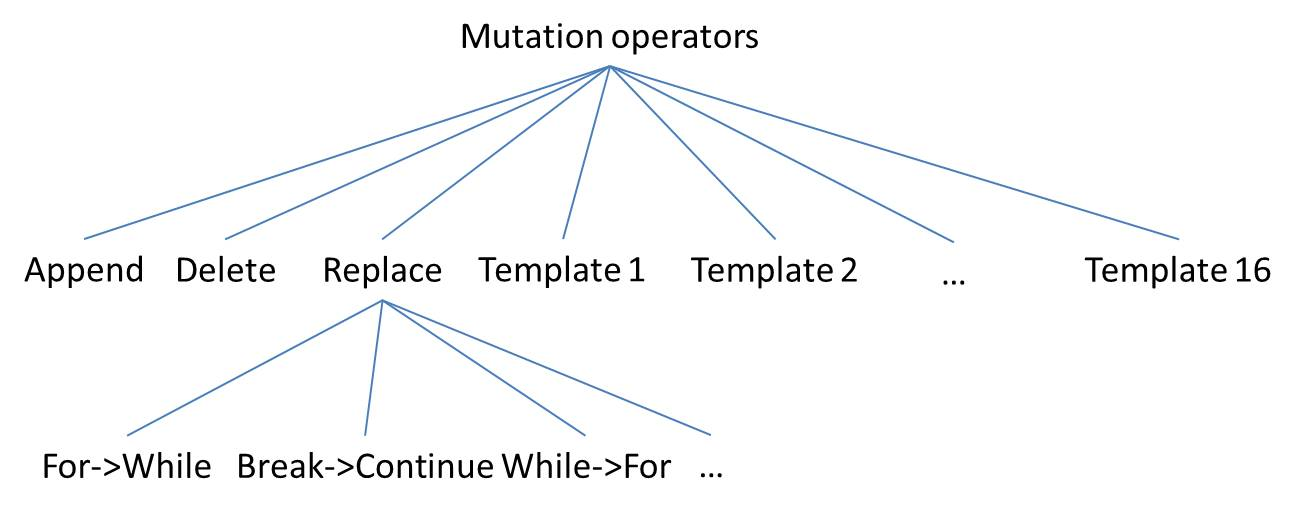
\includegraphics[width=\columnwidth]{Picture2}
  \caption{Two level probabilistic model to inform operator selection and instantiation. \label{fig:probModel}}
\end{figure}

We propose a novel syntactic generate-and-validate repair
technique that differs
from prior work first, in the range of mutation operators considered
(Section~\ref{categorization}) and second, in how it chooses between those
operators and instantiates them.  
We instantiate this technique by extending an open-source implementation of
GenProg~\cite{legoues12} for Java.\footnote{https://github.com/squaresLab/genprog4java}  We add the newly-considered mutation
operators, and a mechanism that allows the tool to
select between the mutation operators according to the probabilities described by
a model.


Our approach uses a two-level model (Figure~\ref{fig:probModel}) in operator
selection/instantiation.  The first level informs the selection of the given
mutation operator, from a set of legal operators at a given potentially-faulty
location (e.g. \emph{Parameter replacer} cannot be applied to a
\emph{BreakStatement}).  If the operator selected is \emph{replace}, the second
level informs the selection of the replacement code.  
To build both models, we perform an incidence count of each mutation operator
and replacement observed in our 
dataset, matched as described in Section~\ref{sec:mining},
and then apply Laplace smoothing~\cite{Russell10} with $\alpha$ = 1 to account
for 0 occurrences.  These two models in detail are as follows: 


\subsubsection{Mutation operator probabilistic model}
The \textit{Mutation operator probabilistic model} 
describes the probabilities of choosing between the several different mutation 
operators at a particular fault location.
%
To build this model,
we count the incidence of each mutation operator observed in our
dataset, matched as described in Section~\ref{sec:mining}. Mutation operator probability is then
weighted accordingly.
%
Figure~\ref{disOfMutOpsTable} describes the distribution of mutation operators
as mined from the corpus. Template-Based and Statement-Edit mutations contribute
29.26\% and 70.74\% of the studied edits, respectively.

\begin{figure}[t]
\centering
\begin{tabular}{lr}
\toprule
Mutation operator & Edits found (\%) \\
\midrule
Append                                                 & 61.03 \\
Sequence Exchance                                      & 15.76 \\
Delete                                                 & 9.10  \\
Param Replacer                                         & 5.93  \\
Param Add/Rem                                          & 3.15  \\
Expression Repl                                        & 1.28  \\
Method Replacer                                        & 1.12  \\
Null Check											   & 0.76  \\
Castee Mutator                                         & 0.61  \\
Replacement                                            & 0.60  \\
Expression Add/Rem                                     & 0.37  \\ 
Cast Check                                             & 0.11  \\
Size Check                                             & 0.07  \\
Range Check                                            & 0.04  \\
Object Initializer                                     & 0.03  \\
Caster Mutator                                         & 0.03  \\
Lower Bound Set                                        & 0.01  \\
Upper Bound Set                                        & 0.00  \\
Off by One                                             & 0.00  \\
\bottomrule
\end{tabular}
\caption{Mined distribution of mutation operators.}
\label{disOfMutOpsTable}
\end{figure}

\subsubsection{Replacements probabilistic model}
If the ``Replacement" mutation operator is 
selected, the \textit{Replacements probabilistic model} describes the probability of replacing one statement (\emph{``replacee"}) with
another (\emph{``replacer"}), thus informing the selection of replacement fix code.
%\footnote{https://goo.gl/mMFbnQ
We consider 
the 22 different types detailed by Eclipse
JDT
%\footnote{AssertStatement, Block, BreakStatement, ConstructorInvocation,
%ContinueStatement, DoStatement, EmptyStatement, EnhancedForStatement,
%ExpressionStatement, ForStatement, IfStatement, LabeledStatement,
%ReturnStatement, SuperConstructorInvocation, SwitchCase, SwitchStatement,
%SynchronizedStatement, ThrowStatement, TryStatement, TypeDeclarationStatement,
%VariableDeclarationStatement, WhileStatement \label{stmtNames}} 
as direct subclasses of the class \texttt{Statement}, and the incidence with which
each 
replaces another. For example: ``What is the observed incidence of a \texttt{For} loop 
replacing a \texttt{While} loop?" Given 22 statement types, there are 484 possible combinations. 
Note that the observed probabilities are not reciprocal, e.g. 
that the probability of a \texttt{For} loop replacing a \texttt{While} loop is different from the 
probability of a \texttt{While} loop replacing a \texttt{For} loop.
This model is built analogously to the
mutation operator model, based on replacer/replacee statement incidence. 


\subsection{Multiple edit association rule mining} 
\label{multEdit}

Although single-edit patches can
repair many non-trivial bugs in real software, the majority of bug fixes in real
software require multiple edits~\cite{zhong15,Soto16}. The number of combinations of possible mutation 
operators to apply in a sequence increases exponentially with number of combined source
code changes.  
%
As a first step towards mitigating this limitation, we propose 
an initial analysis of multi-edit 
source code changes by mining a more expressive model of common changes. In
particular, we extract \emph{association rules}
to model chains of several edits, capturing the way humans create these kinds of fixes.

Association rules are if/then statements that show relationships between elements in a dataset which happen frequently together. We use the 
well-known association rule mining algorithm
Apriori~\cite{Agrawal94}. 
%
We mine association rules for the Mutation operators model
(Section~\ref{sec:modelrepair}) by analyzing mutation operator count in
the studied commits. We develop 
rule sets at different \emph{Confidence} levels, defined as:

\begin{center}
$conf(X \implies Y) = \dfrac{supp(X \cup Y)}{supp(X)}$ 
\end{center}

Where X and Y are items in a transaction (mutation operators, in our
context). Confidence is calculated according to its Support (\emph{supp}), 
an indication of how frequently the set of mutation operators (item set) 
 occurs in the corpus.
Formally:

\begin{center}
$supp(X) = \dfrac{|\{t \in T; X \subseteq t\}|}{|T|}$
\end{center}

Where X is the item set and \emph{t} is each individual transaction in
the database of transactions \emph{T}. Apriori identifies the mutation
operators that frequently happen together in a set of commits, iteratively
extending them to larger 
item sets that appear often in the transactions as identified by these metrics.


\section{Evaluation} \label{evaluation}

We evaluate our model both independently and as part of an automatic repair
technique.  We have four research questions:

\begin{itemize}
\item \textbf{RQ1:} How accurate are our mined models in predicting mutation
  operators and replacement code across a large dataset?
(Section~\ref{sec:generalize})
\item \textbf{RQ2:} Which syntactic operators and selection models are most
  useful for repair? (Section~\ref{sec:oputil})
\item \textbf{RQ3:} How does our model-informed APR tool compare to the
    state-of-the-art in APR? (Section~\ref{sec:comparison})
\item \textbf{RQ4:} What are the most common multi-edit modification rules in
    practice? (Section~\ref{armRes})
\end{itemize}


All experiments are performed on a server 
consisting of 16 processors Intel(R) Xeon(R) CPU E5-2699 v3, with 2.30 GHz each
processor, 46080 KB cache each, and 32 GB RAM memory, operating system Ubuntu 
14.04.5 LTS.  In addition to addressing our research questions as described in
the above roadmap, we provide additional detail on the experimental setup for
all repair experiments in Section~\ref{sec:repairSetup}. 

\subsection{Model generalization}
\label{sec:generalize}
  

%\begin{figure}[ht]
%\tabcolsep=0.18cm
%\begin{tabular}{llllllllllllllllllllll}
%\hline
%As & Bl & Br & Cl & Co & Do & Em & EF & Ex & Fo & If \\
%0\%&2\%&0\%&2\%&5\%&0\%&0\%&0\%&43\%&0\%&22\% \\
%\hline 
%La & Re & SC & Ca & Sw & Sy & Th & Tr & TD & VD & Wh \\
%0\%&0\%&2\%&2\%&0\%&0\%&3\%&2\%&0\%&19\%&0\% \\
%\hline
%\end{tabular}
%\\
%\caption{Example of the Return Statement row of a sub-model created from 
%the training data. Replacee probabillities of the replacer ReturnStatement. The acronyms represent the statement kinds detailed in footnote \ref{stmtNames} \todo{The notes said to remove this, but we can't explain the following section without it, so I am keeping it for now}}
% \label{fig:exPredReturn} 
%\end{figure} 


\begin{figure}[ht]
{\footnotesize
{\centering
\begin{tabular}{l|rrr|rrr}
\toprule
   &\multicolumn{3}{c|}{Replacements} &\multicolumn{3}{c}{Mutation operators} \\
\midrule
Fold	& \# &Prob (\%)& Eq (\%)& \# &Prob(\%)& Eq (\%) \\
\midrule
1	& 155~~&70~~&25~~& 17313~~& 95~~& 64~~   \\
2	& 86~~&100~~&25~~& 17232~~& 93~~& 63~~   \\
3	& 81~~&82~~&23~~& 16754~~& 95~~& 81~~ \\
4	& 101~~&81~~&40~~& 14159~~& 94~~& 9~~   \\
5	& 99~~&90~~&27~~& 17022~~& 95~~& 2~~  \\
6	& 75~~&84~~&21~~& 14945~~& 95~~& 58~~  \\
7	& 79~~&86~~&24~~& 12901~~& 93~~& 7~~  \\
8	& 55~~&96~~&23~~& 10552~~& 95~~& 27~~  \\
9	& 82~~&88~~&8~~& 14568~~& 93~~& 62~~ \\
10	& 116~~&100~~&31~~& 19140~~& 95~~& 6~~ \\
\midrule
Mean	& 92.9 &87.7	&24.7& 15458.6  & 94.3 & 37.9  \\
\midrule
$\sigma$ & 27.4&9.3&	8.0 & 2530.3 & 0.9 & 30.5   \\
%\midrule
%Sum & 1929&877 & 247 &  154586& 943 & 379  \\
\bottomrule
\end{tabular}
\center
  \caption{Correctly predicted edits, across 10 folds of data.
The replacement probabilistic model (center columns, left) predicts
    the correct replacement statement 87\% of the time,
    an improvement of almost a factor of 4 over the equally-distributed equivalent. 
    The mutations model (right columns, left) outperforms the equally-distributed equivalent by 
    almost a factor of 3. \label{results10fcv}} 
}}
\end{figure} 

We begin by independently evaluating our models' (Section~\ref{sec:modelrepair}) predictive accuracy, to
validate the underlying intuition.  We include all Statement-edit and Template-based
mutations, as described in Section~\ref{categorization}.

\subsubsection{Setup}
Our high-level research question concerns whether 
our mined models are likely to identify the correct fix code across a large
dataset, suggesting their potential utility in a repair context.  We therefore
compare the accuracy of the models to an \emph{equally distributed} baseline,
which selects a mutation (or replacement) uniformly at random. This is to contrast 
the accuracy of the priorities assigned by our model to the way it is
performed by current approaches, which pick mutation operators either
uniformly at random, or using coarse grained
heuristics~\cite{legoues12Genprog,kim2013,Qi13TrpAutoR,Weimer13}. 
We measure how often each model correctly predicts the mutation operator (or
replacer statement, for a given replacee statement), within the top 5 produced
choices. Perfect accuracy (correctness in the Top-1 most likely choice) is
unnecessary, since an
APR approach can iterate through several
different candidates before a fix; 
however, the noisy search problem suggests that a relatively tight bound (top-5)
is likely appropriate.

To illustrate, consider a simple example. Assume the following
simple bug-fixing patch from our corpus: 

\begin{lstlisting}[frame=single]
+ if(i > l.size()) {
    return l.get(i); @//original faulty location@
+  }    
\end{lstlisting}

The developer has replaced the original \texttt{return} with an
\texttt{if-then} statement that wraps it.  In assessing the replacement model,
we ask, assuming the selected mutation operator 
is \emph{replace}, how often will an \emph{IfStatement} be predicted as the
replacer for a \emph{ReturnStatement}? If it is returned in the first five
instances in a model, the model correctly predicts this instance.  For the
equally distributed model, we select five operators/replacees uniformly at random. 

We use 10-fold cross validation~\cite{kohavi95} to mitigate the risk
of overfitting and avoid testing and training on the same data.  We aggregate results over
folds by summing the number of correctly predicted instances.

\subsubsection{Results} 

Figure~\ref{results10fcv} shows results.  The \# columns 
show the number of attempted instances per fold.  The ``Prob.'' columns show the
accuracy (correct prediction rate) of the mined model on that fold, for each model; ``EqDist'',
the accuracy of the equally distributed model.  For the Replacements model,
the average accuracy of the Probabilistic model is 63\% higher than the EqDist
model; the difference is 56.4\% for the Mutations model.
Two sample t-tests indicate that both differences in means are statistically significant
($\alpha<0.05$). 

These results suggest that the probabilistic approach is
significantly more accurate than an equally-distributed baseline (used in
several syntactic APR approaches) in predicting bug-fixing edits.  This suggests
that the model, incorporated into an APR approach, may be more likely to produce
correct patches.  We directly address this question next.


\subsection{Repair experiment setup}
\label{sec:repairSetup}

\begin{table}[t]
\centering
  \caption{Studied subjects from Defects4j. \label{defects4j}}
\begin{tabular}{llrr}
\toprule
         &     &            &  Defects\\
 Project & ID & Test cases & considered \\
\midrule
JFreechart & Chart & 2205 & 4\\
Closure compiler & Closure & 7927 & 25\\
Apache commons-lang & Lang  & 2245 & 13\\
Apache commons-math & Math & 3602 & 18\\
%Mockito &	Mockito	 & Mocking framework for junit tests & \todo{I can't find this data} & 0 \\
Joda-Time & Time & 4130 & 3\\
\bottomrule
\end{tabular}
\center
\end{table} 


We have two high-level research concerns related to the utility of our
learned models for repair: 
(1) Which syntactic operators and selection models are most
  useful for repair? (Section~\ref{sec:oputil}) and (2)
How does our model-informed APR tool compare to the
    state-of-the-art in APR? (Section~\ref{sec:comparison})

\paragraph{Validation of models in context} We first compare the utility of the
various sets of syntactic mutation operators to 
identify which sets appears most useful in practice. We
instantiate our tool with each of 
two models (the Equally Distributed baseline from Section~\ref{sec:generalize}
and the learned Probabilistic models), and three different operator sets: (1) Statement-Edit mutations (2)
Template-based mutations, and (3) All mutations. We evaluate each version
for expressive power (in terms of bugs fixed), variants to repair (a machine-
and test suite-independent proxy for time), and quality of the produced patches
(evaluated as described below). 

To diminish the degree of randomness in this experiment and control for the
effect of the mutation probabilities specifically rather than inefficiency and
noise in fault localization, we manually set the fault localization for each
bug. Anecdotally, we observe that less-accurate fault localization increases the
amount of time our tool needs to repair these defects, but does not decrease expressive
power.  

\paragraph{Comparison to previous techniques} Second, we compare our tool, using
the best set of operators as identified in the first question, to four
previously-proposed APR tools: GenProg~\cite{legoues12Genprog}, PAR~\cite{kim2013}, TrpAutoRepair~\cite{Qi13TrpAutoR},
and Nopol~\cite{xuanNopol}. These prior approaches provide coverage over
several dimensions that differentiate program repair techniques.  GenProg and
TrpAutoRepair use the same statement-level edits, but differ in their search
strategies (GenProg uses a genetic programming strategy; TrpAutoRepair, also
known as RSRepair, a random walk). PAR uses GenProg's genetic programming search
strategy, but a different set of templated mutation operators.  Nopol is a
semantics-guided generate-and-validate repair approach that thus uses a fix code
identification strategy that is quite different from the operators we
consider.\footnote{We do not compare directly to
  SPR/Prophet~\cite{long16proph}, because they use machine learning to tune the
  probabilities and rank schema instantiation and are thus
  difficult to re-implement faithfully for Java; as established,
  their edit schemas are generalized by the extended PAR template set.}

The open-source implementation of GenProg for
Java implements  
the first three approaches.   We run these three techniques on the dataset using
parameters described below.  For Nopol, we use patch results released
by the Nopol authors on this same dataset, and do not rerun their experiments.
The Nopol authors have created patches for the same benchmark used in
this study~\cite{martinez2016} and made their results publicly
available.\footnote{\url{https://github.com/Spirals-Team/defects4j-repair/tree/master/results/2017-march}}
We use results from the ``March 2017'' (most recent) release. 

For these experiments, we focus on expressive power (bugs repaired) and
patch quality rather than patch efficiency.  Although important, it efficiency
is not central to our claims, and, given our use of previously-released results,
is difficult to evaluate in a controlled fashion in our context.



\newcommand\mII[1]{\multicolumn{2}{c|}{#1}}

\begin{figure*}\centering
{\footnotesize

\begin{tabular}{l||l|l||rr|rr|rr|rr|rr|rr}
\toprule
 & \multicolumn{2}{c||}{Held-out Test Suite} &\multicolumn{4}{c|}{Statement-Edit Only} & \multicolumn{4}{c|}{Template-based Only} & \multicolumn{4}{c}{All Mutations} \\ 
  \midrule
 \multirow{3}{*}{Bug ID} & \multirow{3}{*}{\shortstack[l]{Held-out\\ tests}} & \multirow{3}{*}{\shortstack[l]{Line \\ coverage}} & \multicolumn{2}{c|}{EqDist} & \multicolumn{2}{c|}{Prob} & \multicolumn{2}{c|}{EqDist} & \multicolumn{2}{c|}{Prob} & \multicolumn{2}{c|}{EqDist} &  \multicolumn{2}{c}{Prob} \\ \cmidrule{4-15}

            &   &  & Time & Quality &  Time & Quality &  Time & Quality&  Time & Quality&  Time & Quality&  Time & Quality \\

\midrule
Closure \#10 & 472 & 60.2\% & 221.0& 100\%  & {179.5} &{100\%} & {175.1}&{100\%} & {121.3}&{100\%} & {163.3}&{100\%} & {157.4}&{100\%} \\
Closure \#18 & 106 & 73.4\% & \mII{No Patch Found} & \mII{No Patch Found} & {36.2}&{100\%} & {197.5}&{100\%} & {45.0}&{100\%} & {139.0}&{100\%} \\
Math \#2     & 13 & 100\%  & \mII{No Patch Found} & \mII{No Patch Found} & {109.4}&{100\%} & {39.6}&{100\%} & {109.4}&{100\%} & {39.6}&{100\%} \\
Time \#19    & 55 & 86\% & 94.1&{100\%} & {80.7}&{100\%} & \multicolumn{2}{c|}{No Patch Found} & \multicolumn{2}{c|}{No Patch Found} & {135.1}&{100\%} & {91.9}&{100\%} \\
Chart \#1    & 93 & 74.4\% & 1.8&{0\%} & {7.3}&{0\%} & {4.9}&{0\%} & {19.0}&{0\%} & {2.2}&{0\%} & {4.8}&{0\%} \\
\bottomrule
\end{tabular}}
\caption{Repair success of various models for three different operator sets.
  Columns 2 and 3 characterize the Evosuite-generated, held-out tests for each
  bug. 
  For each bug, we report time in terms of average variants evaluated to a repair, and
  quality as the percentage of patches created for that bug that pass the
  held-out test suite (an average, if more than one patch is produced over the
  course of multiple random trials). \label{tab:singleLineBugs}}
\end{figure*}

\paragraph{Dataset}
We consider for repair a subset of the Defects4j~\cite{just14}
benchmark, a database and extensible 
framework of real bugs that enables reproducible studies in software testing and
has been previously used to evaluate APR~\cite{martinez2016}. 
Table~\ref{defects4j} characterizes the bugs from the dataset we
consider. Because we compare to single-edit techniques, we 
restrict attention to a subset of the Defects4J bugs with single-line human 
patches.  The number of bugs attempted per project varies based on how many such
bugs are available in the dataset.

\paragraph{Patch quality}
We evaluate patch quality using held-out test
suites~\cite{legoues12Genprog,smith15}.  We automatically generate a single held out suite for each buggy program version that any technique
repairs.  We use Evosuite~\cite{Fraser11Evosuite}, an established 
test suite generation tool for Java, to generate these held-out tests. We run EvoSuite
with a 30-minute budget, using the human-repaired ``after-fix'' version of each Defects4J bug
as the behavioral oracle.  We use
Cobertura\footnote{http://cobertura.github.io/cobertura/} to calculate test
suite 
coverage, again over the ``after-fix'' class that contains the human fix.

\paragraph{Settings} For the genetic programming based techniques (including our own), our population
size is 40, and our max generation size is 10.
For non-GP-based techniques, our maximum considered variant count is 400. For
all techniques, we set a timeout of 4 hours per run.  These settings are
consistent with prior work.  We run 20 seeds per randomized repair trial, in
keeping with recommendations on the assessment of stochastic
techniques~\cite{arcuri11}.

\subsection{Mutation operator and model utility} \label{sec:oputil}

We evaluate our modified APR
techniques, using each of three sets of operators and each of two models to
select between them, on a subset of the bugs in Table~\ref{defects4j}.
Specifically, we consider the first 6 defects from each project. 
Figure~\ref{tab:singleLineBugs} shows results.
The first row (Closure \#10) shows that the
probabilistic model outperforms the equally-distributed model for all three
edit sets.  This happens as well for
Math \#2 and Time \#19, except for the cases where no patch was
found. By contrast, for bugs Chart \#1 and Closure \#18, the equally
distributed approach finds a patch faster on average. Investigating this case
manually, we find that 
these bugs are patched with mutations that are rarely applied by developers (Expression Replace, and Replacement accordingly),
therefore it is more likely that the mutation operators will be chosen by a
random selection than by the developer-informed model.

Our results suggest that considering all available mutation operators is
preferable to 
restricting the mutation operator pool to just one of the categories. For the
Statement-Edit category, 3 out of 6 were fixed faster when combining this kind of mutations with
Template-Based mutations, and 3 out of 6 were slower. For the Template-Based
category: 4 out of 8 were fixed faster when combining it with Statement-Edit
mutations, 2 out of 8 were the same, and 2 out of 8 were slower. This suggests
that the expressive power afforded by an increased set of operators may
outweigh the commensurate increase in search space size, though it is safe to
assume that this benefit must be supported by sufficiently accurate fault
localization. 
%
 %\footnote{\url{https://github.com/mausotog/ReplacementsEmpiricalStudy/tree/master/Randoop10MinHeldOutTestSuites}} 
In this sample, how quickly a model finds a patch appears independent of the mutation
set. 

In terms of
quality assessment, the patches generated behave similarly within a given bug scenario.
That is, for all bugs for which any approach found multiple
patches, either all the patches generated by all configurations
generalized to the held-out test suite, or none did. 

From these results, we conclude that the probabilistic model using all available
mutation operators (both Statement-Edit and Template-based) appears to maximize
expressive power without an unacceptable loss to efficiency.  In conjunction
with our model assessment results (Section~\ref{sec:generalize}), we thus use
all available mutations in our technique for the next experiment. 

\subsection{Comparison to other approaches}
\label{sec:comparison}

\newcommand\mR[2]{\multirow{#1}{*}{#2}}
\newcommand\mCR[2]{\mII{\mR{#1}{#2}}}
\newcommand \mC[1]{\multicolumn{2}{c}{#1}}
 \begin{figure*}
\centering
{\footnotesize
\begin{tabular}{l||r|r||lr|lr|lr|lr|lr}
\toprule
% Full results in https://docs.google.com/spreadsheets/d/1vyD7wH3VGf7X_pUxb4aN9EONO_L_fbIZXw3m9vP7MRc/edit#gid=0
\multirow{3}{*}{Bug ID} & \multirow{3}{*}{Held-out tests} & \multirow{3}{*}{Line coverage} & \mII{Prob. Model} & \mII{GenProg} & \mII{TrpAutoRepair} & \mII{PAR} & \mC{Nopol} \\\cmidrule{4-13}
       &  &  & Found & GTHTS & Found & GTHTS &Found & GTHTS &Found & GTHTS &Found & GTHTS   \\ 
\midrule
Chart \# 1 & 93 & 74.4\% & 5 & 0\% & 6 & 0\%  & 4 & 0\% & 2 & 0\% & \multicolumn{2}{c}{No Patch Found}   \\
Closure \# 10 &  472 & 60.2\% & 2 & 100\% & \mII{No Patch Found}  & \mII{No Patch Found} & \mII{No Patch Found} & 1 & 100\%   \\
Closure \# 18 & 106 & 73.4\%      & 1 & 100\%    & \mII{No Patch Found}  & \mII{No Patch Found} & \mII{No Patch Found}  &1 &  100\%  \\
Closure \# 86 & 435 & 64.8\% & 2 & 100\% & \mII{No Patch Found}   & 1 & 100\% & \mII{No Patch Found}  & \multicolumn{2}{c}{No Patch Found}   \\
Lang \# 33 &  85 & 92.3\%  & 1 & 100\% &  \mII{No Patch Found}   &   \mII{No Patch Found}  &1  & 100\% &   \multicolumn{2}{c}{No Patch Found}   \\       
Math \# 2  & 13 & 100\%  & 1 & 100\% & \mII{No Patch Found} & \mII{No Patch Found} & 1 & 100\% & 1 & 100\%  \\
Math \# 75 &  25 & 92.5\%      & 1 & 100\%    & \mII{No Patch Found}  & \mII{No Patch Found} & 1 & 100\%     & \multicolumn{2}{c}{No Patch Found}   \\
Math \# 85 & 11 & 94.7\% & 4 & 0\% & 8 & 0\%  & 3  & 0\% & 8 & 0\% & 1  & 100\%  \\       
Time \# 19 & 55 & 86\%  & 2 &100\% & 1 &100\% & 1 & 100\%& \mII{No Patch Found} & 1 &  100\% \\
\bottomrule
\end{tabular}}
  \caption{Comparison between the probabilistic model-based repair and other state-of-the-art 
  approaches. The ``Found" column represents the number of patches found for this bug. Because 
  each randomized technique is run several times, some techniques find multiple patches per bug. 
  The ``GTHTS" column represents the percentage of these patches that Generalized To a Held-out 
  Test Suite. \label{stateOfTheArtComparison}} 
\end{figure*}


Next, we use our new APR approach to attempt to repair the
defects described in Table~\ref{defects4j}, comparing to other state-of-the-art
approaches. 
Figure~\ref{stateOfTheArtComparison} shows
results for the subset of bugs that our technique repairs (in the interest of
space, we describe results
for the remaining bugs in prose below). 
Figure~\ref{stateOfTheArtComparison} shows the number of unique patches found
for each bug and how many of them generalized 
to a held-out test suite. The patches that did not generalize failed one or 
several tests in the held-out test suite. Of the
19 distinct patches created by our approach, 
10 pass all held-out test suite (52.6\%); 
6.6\% of GenProg's patches generalize; 22.2\% of TRPAutoRepair's;
23.1\% of PAR's; and 100\% of the 5 Nopol patches generalize to the held-out test suite.
One example demonstrating the quality provided by the probabilistic
model-based approach is seen in the Closure \#18 bug; Figure~\ref{closure18prob} 
shows our technique's patch, identical to the human patch.

\begin{figure}[t]
\begin{lstlisting}[firstnumber=1287][frame=single]
boolean staleInputs = false;
@-if(options.dependencyOptions.needsManagement() && options.closurePass){
+if(options.dependencyOptions.needsManagement()){
@  for (CompilerInput input : inputs) {
    // Forward-declare all the provided types, so that they
    // are not flagged even if they are dropped from the process.
    for (String provide : input.getProvides()) {
      getTypeRegistry().forwardDeclareType(provide);
    }  
  }
	\end{lstlisting}

	\caption{A patch generated using the probabilistic model, identical to the
      developer patch; No other approach found this identical patch.\label{closure18prob}}
\end{figure}

A key takeaway from these results is that the probabilistic approach outperformed all the heuristic
approaches.  This is important because these approaches by construction select
syntactic edits to perform according to some distribution.  That is, these techniques are those that \emph{could}
benefit from a more informed edit distribution model.  
By contrast, Nopol produced 5 patches that all generalized to the held out test suite.  However, Nopol
targets a specific bug type and does not use a 
heuristic approach.  Our approach therefore presents an important benefit for a
broader array of bug types, particularly those to which a semantics-based
approach like Nopol doesn't apply. Overall, these results demonstrate the
benefit of applying a probabilistic model for edit selection for those
approaches to which such a selection process applies. 

Our technique patched 9 of the 63 bugs in our evaluation. 
GenProg patched 9; Par, 16; Nopol, 27; and TRPAutoRepair, 8. There are 37 bugs for which at least one of the five evaluated approaches obtained a 
patch. From these, 19 were patched by only one approach; 10 were patched by 
two; 3 patched by three; 4 patched by four; and 1 patched by the five evaluated approaches.

Many approaches can create several patches for each bug. 
Our approach created 19 distinct patches for the aforementioned 9 bugs.
Of these, 10 (52.6\%) pass the held-out test suites.
Genprog created 46 distinct patches; 5 of them (10.9\%) pass the test suites.
TRPAutoRepair created 30 patches; 4 of them (13.3\%) pass the test suites.
PAR created 34 patches; 11 of them (32.4\%) pass the test suites. 
Finally Nopol created 28 patches; 21 of them (75.0\%) pass the test suites.

\subsection{Association Rule Mining} \label{armRes}

In this section, we
describe and evaluate the mutation operator association rules produced by
mining human patches to identify edits that commonly occur together in
human-generated patches (Section~\ref{multEdit}).  The goal of these models is
to provide intuition regarding how to form multi-edit source code changes.  Note
that we create these association rules using strictly the Mutation Operator
model corpus; the Replacements operator corpus is only informative when the
``Replace'' operator is chosen, and thus does not apply to the
question of chaining together edits to produce larger patches.

\subsubsection{Mutation operator rules} \label{mutOpRules} Below, we list the
top 10 rules identified with 100\% confidence in the dataset. This means that in
100\% of the cases observed, every transaction that contained the antecedent of
a rule also contained the consequent. A high threshold like 100\% produces
rules for APR that predict with high accuracy which edits to perform, given an
initial set of edits.  These rules are obtained with a 1\% support, which means that
each of these rules individually appear in at least 1\% of all the transactions
in the corpus. We show only the top
association rules, and also release the full set of mined rules to inform future
studies in multi-edit repair:\footnote{https://github.com/squaresLab/ProbabilisticModelSaner2018}
%\footnote{\url{https://github.com/mausotog/ReplacementsEmpiricalStudy/blob/master/ResultsAssociationRuleMiningMutOperators.txt}} 

%Minimum support: 0 (1 instances)
%Minimum metric <confidence>: 0.9
%Number of cycles performed: 20
\hfill
\begin{itemize}
 \item Replace \& Delete $\implies$ Append
 \item Delete \& AddNullCheck $\implies$ Append
 \item Replace \& SeqExchanger $\implies$ Append
 \item Replace \& ParamReplacer $\implies$ Append
 \item Delete \& CasteeMutator $\implies$ Append
 \item Replace \& Delete \& ParamReplacer $\implies$ Append
 \item Replace \& AddNullCheck $\implies$ Append
 \item Replace \& Delete \& SeqExchanger $\implies$ Append
 \item Delete \& ExpressionAdder $\implies$ Append
 \item Delete \& AddNullCheck \& ParamReplacer $\implies$ Append
\end{itemize}
\hfill

The key observation to draw from these rules is that ``Append'' is the most
common single edit mutation operator applied by 
developers. This behavior is reflected in the fact that it is the consequent in
all the top mined rules.
Overall, association rules provide an intuition of which common patterns of behavior
developers use. These rules tell us what edits happen frequently together, which
will help us further understand multi-edit source code changes, an understudied 
area that covers the majority of real life patches.

\subsubsection{Evaluation of Association Rules}
To evaluate the effectiveness of the association rules in the context of the
automatic program repair process, we first remove from the corpus human patches
with fewer than three edits.  This is because 
our mined rules all require at least two
antecedents and one consequent. This removed 62.83\% of the
corpus. We validated the rules on the remaining 37.17\% of patches as follows.
First, we divide our 
corpus in 10 folds. For each fold, we build association rules on the remaining
nine, as described. Given the mined rules, we then we
analyze how many testing patches (instances in the fold used as testing data) can be
built by applying the learned rules.  We categorize them as either
\emph{Fully covered}, \emph{Partially covered}, or \emph{Not covered}.

To illustrate via example, 
Table~\ref{rulesandinstances} shows three instances of patches in the testing
data, and three rules. Instance 1 can be constructed by
applying rules 1 and 3 and is thus classified as Fully
covered. Rule 1 would cover the first three edits of Instance 2
instance, but there is no way to create the Replace (``Rep'') mutation using the
listed rules.  This instance is classified as Partially covered. For Instance 3,
even though Rule 3 
contains two of the edits in the rule's antecedent, the instance does not
contain the rule's consequent.  The rules do not apply, and thus this instance
is classified as Not covered.

\begin{table}[ht]
  \centering
  \caption{Patch instances (top); associated association rules (bottom). \label{rulesandinstances}}{\small
\begin{tabular}{ll}
\toprule
\multicolumn{2}{c}{Instances} \\
\midrule
1 & Del; App; NullCheck; ObjInit \\
2 & Del; App; NullCheck; Rep \\
3 & App; NullCheck; CastMut \\  
\midrule
 \multicolumn{2}{c}{Rules} \\                     
\midrule
1 & Del $\wedge$ App $\rightarrow$ NullCheck \\  
2 & App $\wedge$ ParamRep $\rightarrow$ Rep \\   
3 &App $\wedge$ NullCheck $\rightarrow$ ObjInit\\
\bottomrule
\end{tabular}

}
\end{table}

Finally, we performed this analysis at 6 different confidence thresholds
(50\%, 60\%, 70\%, 80\%, 90\%, 100\%) to analyze the tradeoff between ruleset expressive
power and size. A high confidence produces 
a small number of very accurate rules (when the
antecedent is present, it is very likely that the consequent will be present as
well).  Setting the confidence lower produces the opposite trade-off:
a large set of rules (covering more instances) where if the antecedent is
present, it is less likely that 
the consequent will be present too. For each confidence
threshold, we performed a standard 10-fold cross validation process with all the
instances and all the rules for each fold and finally, we aggregate the results
from all the folds.

\begin{comment}
\begin{table}[ht]
\centering

\begin{tabular}{|c|rrrr|}
\toprule
 Confidence(\%) & Rule count & Fully Cov & Partially Cov & Not Cov \\
\midrule
100 & 185.4 & 119.9 & 3.2 & 194.8 \\
90 & 251.4  & 269.3 & 4.5 & 44.6 \\
80 & 358.2  & 290.5 & 4.7 & 23.2 \\
70 & 438.7 & 298.7 & 5.9 & 13.8 \\
60 & 551.8 & 304.4 & 6.6 & 7.4   \\
50 & 701.8 & 310.0 & 5.9 & 2.5 \\
\bottomrule
\end{tabular}
\center
  \caption{10-fold cross validation with different confidence thresholds. \label{10FoldXValResults}}
\end{table} 
\end{comment}


\begin{figure}[!h]
  \centering
    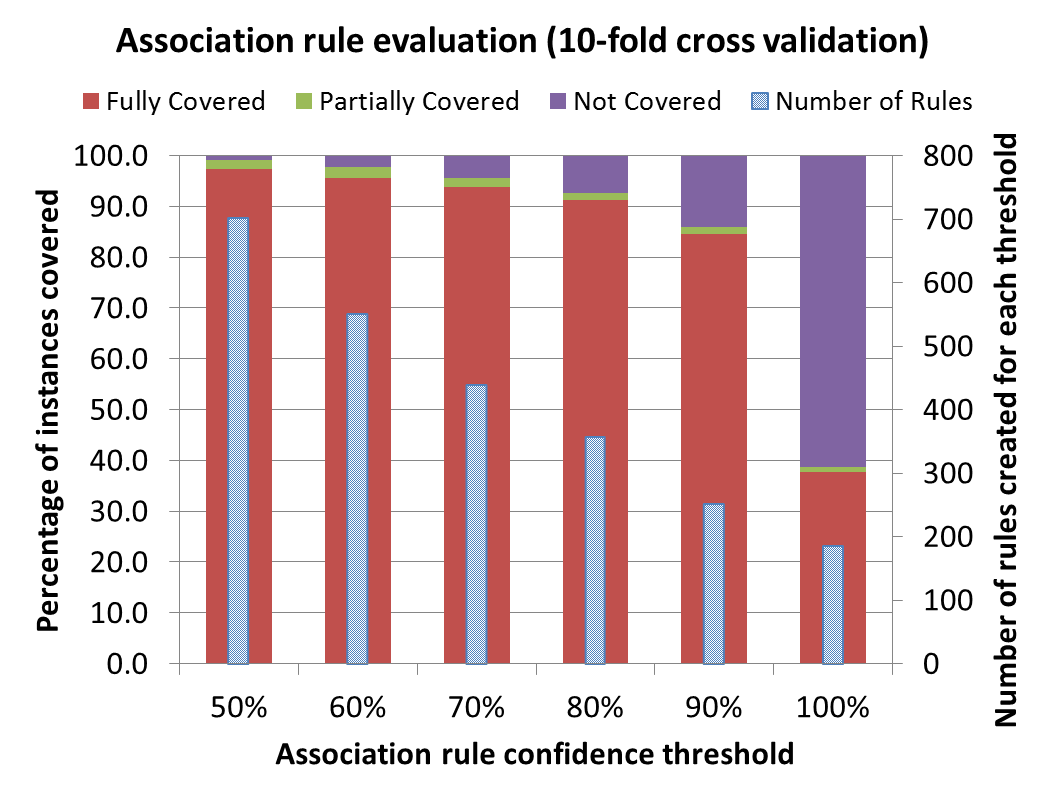
\includegraphics[width=\columnwidth]{10FoldXVal4}
  \caption{The wide bars use the left vertical axis to describe the percentage of patches covered (Fully, Partially or Not) by the association rules. The thin bars use the right vertical axis to describe the number of rules created for each confidence threshold.}
  \label{fig:assocRulesEvaluation}
\end{figure}

Figure~\ref{fig:assocRulesEvaluation} shows results.  As expected, the number of rules created
increases as confidence decreases.  Note also that the
number of Fully Covered instances increases as the confidence decreases, due to
the fact that there are more rules, even though these rules are less accurate.

APR would benefit from having a small number of very accurate (high confidence)
rules that would describe what edit to perform next after a series of edits, but
at the same time, it needs rules that are flexible enough that they can
generalize to a big portion of the patches.
%
We find that a good tradeoff within this tension happens when we set the
confidence threshold to 90\%. There is a big difference between 100\% and 90\%
confidence thresholds regarding percentage of Not Covered. The 100\%
threshold provides very accurate rules, but can fully cover only a
37.7\% of the patches it was evaluated on. By contrast, the 90\% confidence
threshold produces slightly more rules, but the rules generalize much
more and are able to fully cover 84.6\% of the patches, while 
still maintaining a high confidence threshold.



\section{Threats to Validity} \label{threatsVal}

\noindent\textbf{Internal validity:}
Regarding possible errors in our implementation and experiments, to run our
comparison with Genprog, we used an open-source implementation of GenProg
targeting Java. We release our code, as well as our templates,
independently-generated tests, and mined models for scrutiny and extension by other
researchers, to mitigate the risk of errors in our implementation or approach. 
 We also use 10-fold cross validation in
assessing our model and association rules, to reduce the risk of training and testing on the same
data.  
%REMOVE THIS FOR CAMERA READY
%in the project mentioned before 

\noindent\textbf{External validity:} 
It is possible 
that our results will not generalize to external datasets and to
real bugs. To mitigate this concern, we build our model from well-known open-source
programs, covering a diversity of applications, and distinct from the dataset
from which the models were mined, and we evaluate our approach with bugs from an open-source framework.

There is also risk of producing low quality patches that would not 
generalize
to a different description of desired program behavior. We attenuate 
this by 
assessing the quality of the generated patches with a held-out test suite.
There is risk in the fact that we are manually giving the
faulty location to the APR tool, since APR tools do not know in advance what the 
fault location is. This is for the purposes of evaluating the patch creating 
process
only without the noise that fault localization might introduce.

\noindent\textbf{Construct validity:}
Regarding the suitability of our evaluation metrics, we evaluate patch
quality by running the generated patches on a second test suite created
from a human patch, which is to a certain extent a biased measure since we can
not guarantee that the human created patch is perfect~\cite{smith15}. Nevertheless, we consider 
this to be a
best known practice, since this way we provide an alternative to subjectively 
asking a biased human developer
whether he/she considered the patch to be correct or not. 

We also rely on Evosuite~\cite{Fraser11Evosuite} as our test suite generation
mechanism for the held-out test suite used for evaluation, and we acknowledge
that the test suites created by this tool may not be perfect, nor provide full
coverage for all cases.  Nonetheless, this is a state-of-the-art test suite
generation tool that mitigates the risk of bias in manually constructing
evaluation test suites.

\section{Related Work} \label{relatedWork}

There have been previous efforts to create an edit model based on human behavior.  
Soto et al.~\cite{Soto16} 
built a probabilistic model to describe the replace 
operator only. They do not evaluate the model in the context of a repair
tool, and the model is based on an instance count of statements rather than a more 
accurate analysis of AST differences, which our model was built from.  
HDRepair~\cite{xuan16} 
uses fix history
to assess patch suitability and fitness in the context of a genetic
programming search strategy. The fitness of the generated
fix candidates is determined by the frequency with which the changes included in
a given patch occur in the corpus, using a graph-based representation of the bug
fixes.  Similarly, Prophet~\cite{long16proph} uses a
probabilistic model of a subset of our considered mutation operators built on 
the history of 8 different projects to rank candidate
patches.  Our approach follows this intuition to mimic human
behavior; unlike the previous work, we apply this knowledge when actually
creating patch candidates rather than when evaluating them, which reduces the 
search space at creation time.  

Zhong and Su~\cite{zhong15} perform an empirical study of
real bug fixes on six projects, studying the incidence of three mutation
operators, among other questions about the applicability of APR.  Martinez and
Monperrus~\cite{martinez15} similarly study mutation operator incidence across 
14 
projects. Our work considers a broader set of
mutation operators over a larger corpus, the largest, to the best of our
knowledge, studied in existing work. To counter the 
risk of overfitting to a small set of training projects as performed before, our 
current study trains the model over 500 projects, covering a diversity 
of domains.

Par~\cite{kim2013} describes a manual set of 10 templates of common behavior to
create patches, showing that such templates result in patches of higher
human-adjudged acceptability than statement-edit-based patches.  Our study takes 
into consideration a superset
of these templates, provides steps towards
accounting for multi-edit source code changes, an understudied problem, and,
importantly, mines and models these operators and their incidence automatically
(rather than manually).

There exist a broad array of APR techniques proposed, especially recently; we
survey many of them in Section~\ref{background}, focusing on heuristic or
syntactic generate-and-validate techniques.  Semantic-based techniques use
semantic analysis or reasoning~\cite{nguyen13,mechtaev15,Mechtaev2016,Bach17S3}, or
semantic search~\cite{ke15} to construct candidate patches.  Similarly,
synthesis-based repair is a family of techniques that uses constraints to build
patches following the description of the constraints~\cite{jin11,wei10}. These constraints may be
specifications created by developers, formal verification, invariants,
etc.~\cite{jin11,wei10}.  Such techniques typically use synthesis to construct
repairs, with a different mechanism for both constructing and traversing the
search space, and our approach is thus less immediately comparable.
 

\section{Conclusion} \label{conclusion}

In this paper, we analyze the way in which current state-of-the-art automatic 
program repair approaches select mutation operators to create candidate 
patches. We analyze, categorize and compare the mutation operators being used by 
state-of-the-art approaches. We analyzed the last 100 bug fixing commits from 
the
500 most-starred Java projects on GitHub, which is the largest corpus analyzed
to date, to the best of our knowledge. We picked the most-stared projects because stars in Github are seen as proxies for popularity, which usually entail well-maintained, well-stablished, mature projects, that are more likely to have more and better quality bug fixes. We created a two-level probabilistic 
model describing
the likelihood of selecting bug-fixing mutation operators, according to the
observed incidence of their use by human developers. All the data gathered, 
tools and test suites used in this study are publicly available for open peer review 
and scrutiny.

We evaluated our approach in several ways: by performing an internal 
evaluation of 
its predictive power, and by
 running an APR tool using our model on 63 bugs from
Defects4j. Finally we compare the quality of the patches 
generated against patches created for these same bugs by other state-of-the-art 
approaches. We measure both efficiency of patch production, and generalizability
of the patches to a held-out test suite.  
Note that in Figure~\ref{tab:singleLineBugs}, for the majority of bugs, when using the probabilistic
model we obtained better results than their equally distributed 
counterpart.
Overall, we found that automatic program repair appears to benefit
from having a diverse mutation operator pool; future improvements in fault localization thus will
serve to further benefit from more precise models of mutation selection. 

Multi-edit source code changes are understudied, but cover
a large portion of bug fixes in software systems. 
To move towards advancing this area, we constructed a set of association rules 
that describe 
how subsets of mutation operators are applied together.
%
Overall, our initial analysis of how to chain single-edit changes by following
human behavior provides a critical
first step towards an efficient mechanism for traversing the large search space
of multi-edit repairs by showing that we can construct a large percentage of the corpus from the created rules while maintaining a 90\% confidence threshold.




% conference papers do not normally have an appendix


% use section* for acknowledgment
\section*{Acknowledgments}

This work partially supported by the National Science Foundation (under award
CCF-1563797) and the Air Force Research Laboratory (AFRL Contract
No. FA8750-15-2-0075). Any findings or recommendations are those of the
author(s) and do not necessarily reflect the views of the sponsoring agencies.
The authors additionally wish to thank the anonymous reviewers, whose comments
were particularly constructive.



% trigger a \newpage just before the given reference
% number - used to balance the columns on the last page
% adjust value as needed - may need to be readjusted if
% the document is modified later
%\IEEEtriggeratref{8}
% The "triggered" command can be changed if desired:
%\IEEEtriggercmd{\enlargethispage{-5in}}

% references section

% can use a bibliography generated by BibTeX as a .bbl file
% BibTeX documentation can be easily obtained at:
% http://mirror.ctan.org/biblio/bibtex/contrib/doc/
% The IEEEtran BibTeX style support page is at:
% http://www.michaelshell.org/tex/ieeetran/bibtex/
%\bibliographystyle{IEEEtran}
% argument is your BibTeX string definitions and bibliography database(s)
%\bibliography{IEEEabrv,../bib/paper}
%
% <OR> manually copy in the resultant .bbl file
% set second argument of \begin to the number of references
% (used to reserve space for the reference number labels box)
%\begin{thebibliography}{1}

%\bibitem{IEEEhowto:kopka}

%\end{thebibliography}

\bibliographystyle{abbrv}
\bibliography{sigproc}  % sigproc.bib is the name of the Bibliography in this case
% You must have a proper ".bib" file
%  and remember to run:
% latex bibtex latex latex
% to resolve all references



% that's all folks
\end{document}


